\documentclass[english,11pt]{beamer}

\DeclareMathOperator{\Cov}{Cov}
\DeclareMathOperator{\Var}{Var}
\DeclareMathOperator{\E}{\mathbb{E}}
\DeclareMathOperator{\Proba}{\mathbb{P}}

\newcommand{\Covb}[2]{\ensuremath{\Cov\!\left[#1,#2\right]}}
\newcommand{\Eb}[1]{\ensuremath{\E\!\left[#1\right]}}
\newcommand{\Pb}[1]{\ensuremath{\Proba\!\left[#1\right]}}
\newcommand{\Varb}[1]{\ensuremath{\Var\!\left[#1\right]}}

% norm
\newcommand{\norm}[1]{\| #1 \|}

\newcommand{\indep}{\rotatebox[origin=c]{90}{$\models$}}





\usepackage{mathptmx,amsmath,amssymb,graphicx,bibentry,bbm,babel,ragged2e}

\makeatletter

\newcommand{\noun}[1]{\textsc{#1}}
\newcommand{\jitem}[1]{\item \begin{justify} #1 \end{justify} \vfill{}}
\newcommand{\sframe}[2]{\frame{\frametitle{#1} #2}}

\newenvironment{centercolumns}{\begin{columns}[c]}{\end{columns}}
%\newenvironment{jitem}{\begin{justify}\begin{itemize}}{\end{itemize}\end{justify}}









%\usetheme{Warsaw}
%\setbeamertemplate{footline}[text line]{}
%\setbeamercolor{structure}{fg=purple!50!blue, bg=purple!50!blue}
%\setbeamersize{text margin left=15pt,text margin right=15pt}




\usetheme{Boadilla}


% redefine palette
\definecolor{cybblue}{HTML}{1C6F91}


\setbeamercolor{structure}{fg=cybblue}

\setbeamercovered{transparent}


\addtobeamertemplate{title page}{%\hspace{-0.4cm}
\vspace{-0.8cm}
\hspace{-0.5cm}
%\includegraphics[height=1.2cm,width=1.2\textwidth]{template/bandeau3}\\
}{%
%\begin{textblock*}{150mm}(-1cm,-1.5cm)
%\end{textblock*}
}


\setbeamertemplate{footline}{
\hspace{0.2cm}
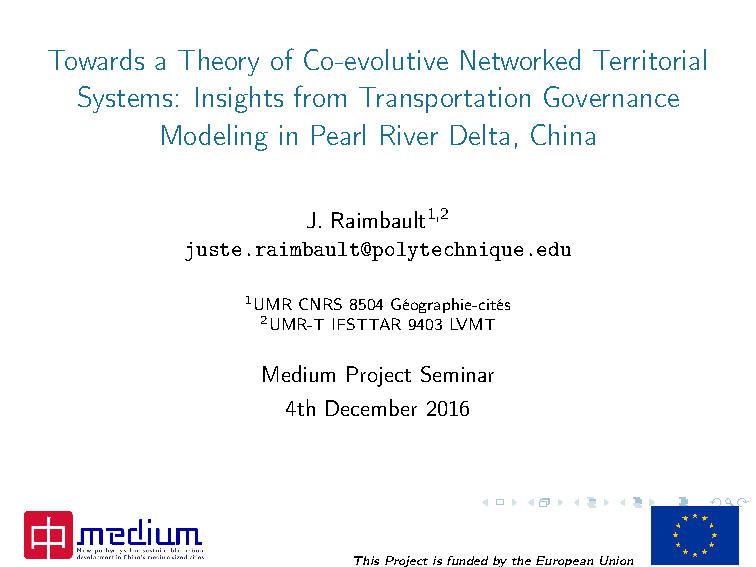
\includegraphics[height=0.75cm]{template/medium}
\hfill
\includegraphics[height=0.75cm]{template/eu}
\hspace{0.15cm}
\vspace{0.15cm}
}





\@ifundefined{showcaptionsetup}{}{%
 \PassOptionsToPackage{caption=false}{subfig}}
\usepackage{subfig}

\usepackage[utf8]{inputenc}
\usepackage[T1]{fontenc}


\usepackage[usenames,dvipsnames]{pstricks}
\usepackage{epsfig}



\makeatother

\begin{document}


\title{A Macro-scale Model of Co-evolution for Cities and Transportation Networks}

\author{J.~Raimbault$^{1,2}$\\
\texttt{juste.raimbault@polytechnique.edu}
}


\institute{$^{1}$UMR CNRS 8504 G{\'e}ographie-cit{\'e}s\\
$^{2}$UMR-T IFSTTAR 9403 LVMT\\
}


\date{Medium 2017 Conference\\\smallskip
\textit{Spatio-temporal Behavior in Complex Urban Systems}\\\smallskip
17th June 2017
}


{


\setbeamertemplate{footline}{
\hspace{0.2cm}
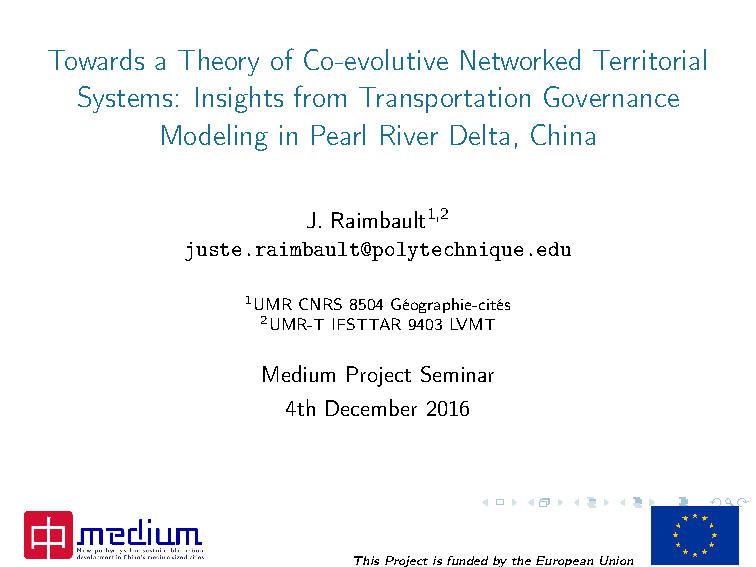
\includegraphics[height=1cm]{template/medium}
\hfill
\textit{This Project is funded by the European Union}\hspace{0.2cm}
\includegraphics[height=1cm]{template/eu}
\hspace{0.2cm}
\vspace{0.5cm}
}


\frame{\maketitle}

}




%%%%%%%%%%%%%%%%%%%
%% ABSTRACT

%The complexity of Urban Systems is closely linked to the co-evolutive character of their different components or agents (Pumain, 1997). In the case of cities and transportation networks, this co- evolution has been shown empirically (Bretagnolle, 2007) but remains poorly understood in terms of its dynamical processes. We introduce a model of spatial interactions between cities at the macro-scale, in the spirit of stochastic urban growth models inheriting from the Gibrat model (Favaro and Pumain, 2011). We include evolving transportation networks, in order to explore stylized hypothesis on the interactions and drivers of the growth of both network and cities. In a multi-modeling fashion, the model can take into account various processes such as between cities direct interactions, network-mediated interactions, feedback of network flows, and for the network demand-induced growth. The latter is tested at different abstraction levels that are the time-distance matrix between cities, and physical network growth trying to satisfy greedy time-gain optimization criteria. We use as a benchmark network the geographical shortest paths that have been shown in a previous work to already capture network effects (Raimbault, 2016). The model is tested and explored on synthetic city systems, generated following a simple heuristic to follow the rank-size law and Central Place Theory. The systematic exploration through intensive computation unveils different interaction regimes accross the parameter space. In some, the introduction of the network can drastically change the fate of some cities, whereas the top-distribution hierarchy is reinforced, what is consistent with empirical observations in the literature. Some regimes actually exhibit circular causalities between network and city growth, corresponding to the intricated co-evolution. The model will be applied to the French Urban System on long time dynamical data (Pumain-INED database for populations spanning between 1831 and 1999, with the evolving railway network from 1850 to 2000, and a specifically-designed database of the highway networks containing its full genesis from 1950 to 2015), and to the Chinese Urban System after 2000 with the High Speed Rail (HSR) network, both realized and planned. Expected results concern both accurate city population growth reproduction, and network patterns, i.e. how does taking into account dynamical networks can introduce further exploratory power in such models, and reciprocally how can such coupled models produce realistic networks compared to more classical autonomous models of network growth. The role of medium-sized cities on the trajectories of the system can also be examined with the model. Finally, a comparison between the urban systems in different geographical and political contexts and at different scales should unveil implications of planning on the interactions between networks and cities, for example by comparing the rather bottom-up growth of the French railway network to the top-down state-planned French highway and Chinese HSR networks.




%%%%%%%%%%%%%%%%%%%
\section{Introduction}
%%%%%%%%%%%%%%%%%%%


\sframe{Systems of Cities and Transportation Networks}{

\centering

\textit{(Left) Hong-Kong-Zhuhai-Macao Bridge ; (Right) Near XiaoLan station}

\medskip

\includegraphics[width=0.48\textwidth,height=0.5\textheight]{figures/hzmb}\hspace{0.2cm}
\includegraphics[width=0.48\textwidth,height=0.5\textheight]{figures/xiaolan}

{\tiny Source - Left : http://www.hzmb.hk ; Right : Photo by author}

}


\sframe{Co-evolution}{

\justify

% what is the co-evolution, why model it, what model exist (include our other works)

\footnotesize

\vspace{-0.3cm}

$\rightarrow$ Co-evolution between networks and territories shown empirically \cite{bretagnolle:tel-00459720}

$\rightarrow$ Models endogeneizing it are very rare ; possible explanation : interdisciplinary question and compartmentalization of disciplines~\cite{raimbault2015models}

$\rightarrow$ Diverse precursor approaches: LUTI models~\cite{wegener2004land}; Network Growth (Geometrical \cite{courtat2011mathematics}, Economical \cite{xie2009modeling}, Biological \\\cite{tero2010rules}) 

% include citation network (sexy)

%\smallskip
\centering

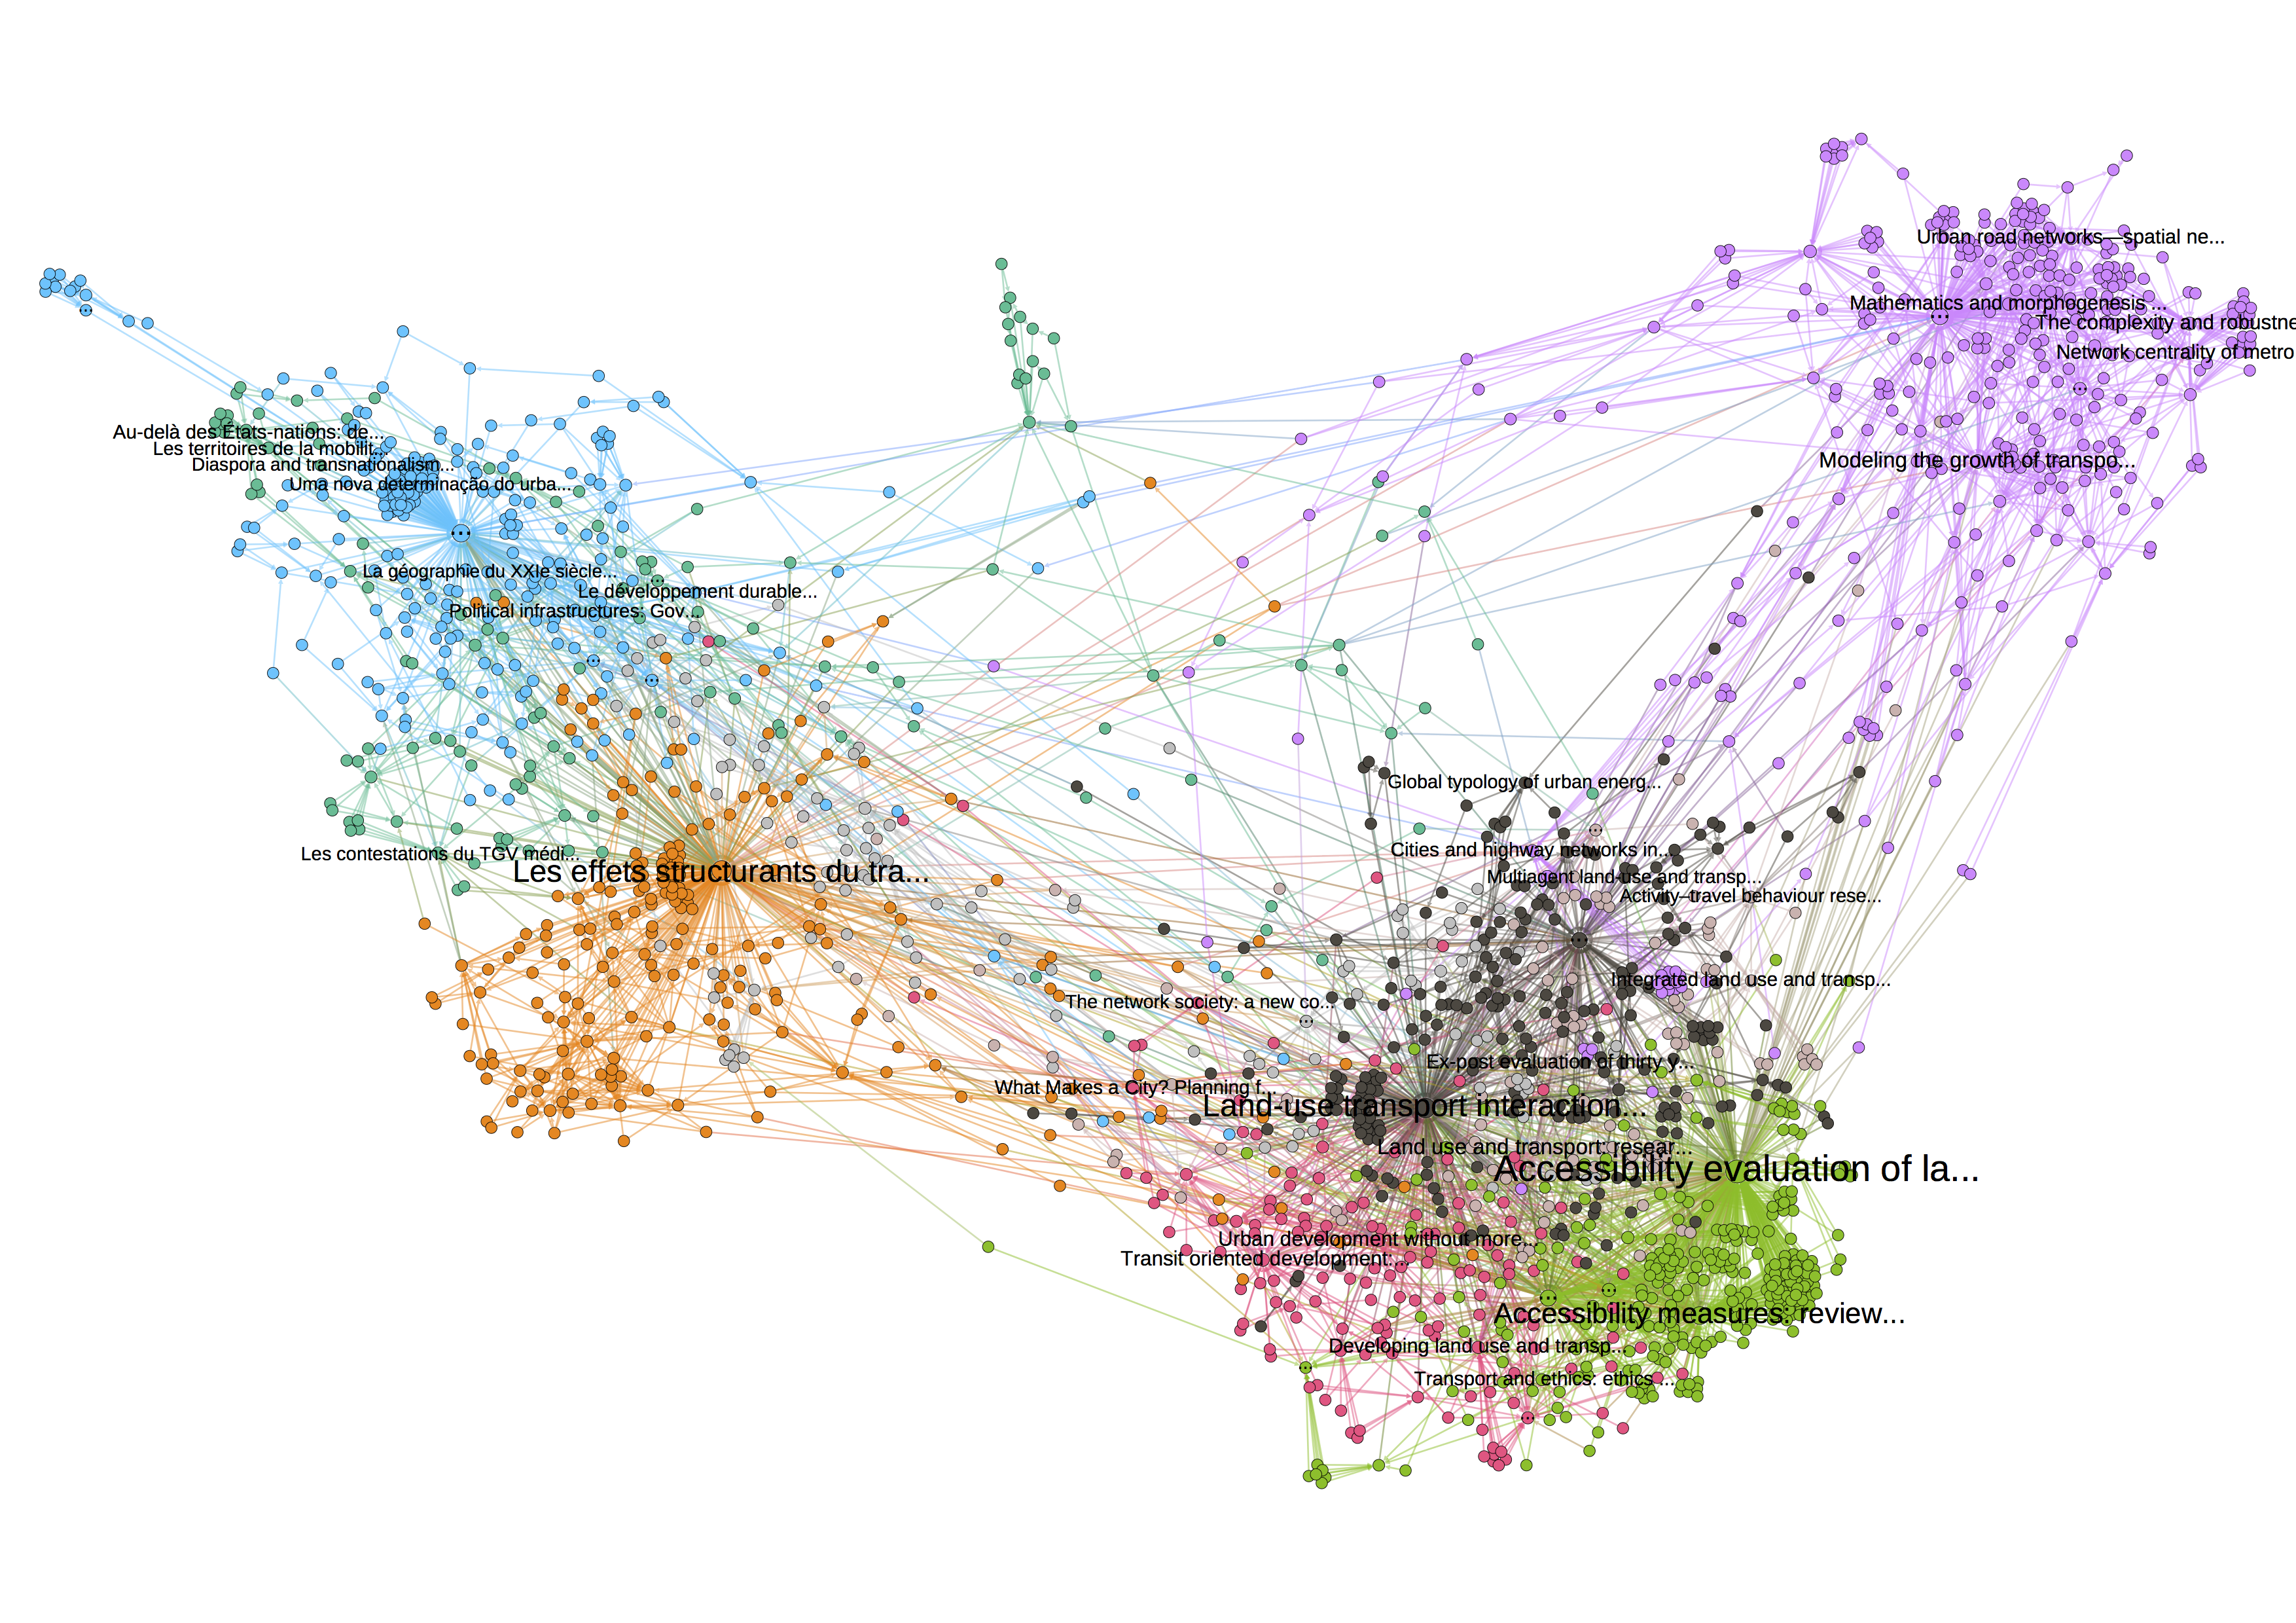
\includegraphics[height=0.6\textheight]{figures/rawcore}

{\footnotesize\textit{Multidisciplinary citation network for studies of relations between networks and territories}}

}


\sframe{Towards Models of Co-evolution}{

% question / objective

\justify

\textbf{Why model it ?} \textit{Insights into dynamical processes in System of Cities ; Perspective of Operational Models}

\medskip

\textbf{Several possible Scales and Ontologies}

\begin{itemize}
\item Micro-scale: mostly chaotic regimes, too precise for reasonable models (shown for traffic by~\cite{raimbault2017investigating})
\item Meso-scale: Urban Form, Accessibility and Network Shape \cite{raimbault2017models}
 ; Transportation Governance in Mega-city Regions~\cite{le2015modeling}
\item Macro-scale: SimpopNet model~\cite{schmitt2014modelisation}
\end{itemize}

\medskip

\textbf{Research Objective}

$\rightarrow$ \textit{Introduce a parsimonious but modular model of co-evolution of cities and networks at the scale of a System of Cities.}




% speak quickly of mesocoevol / Lutecia.

}

\sframe{Submodel coupling}{

\centering

% incl. schema on what is a strongly coupled co-evolutive model

\includegraphics[height=0.9\textheight]{figures/coevolution.pdf}


}



%%%%%%%%%%%%%%%%%%%
\section{Model and Results}
%%%%%%%%%%%%%%%%%%%


\sframe{Model : Rationale}{
  % - explain choices, funding literature etc.
  % - considerations on randomness ; comparison with Simpopnet
  
  \justify
  
  \textbf{\textit{Interaction between cities at different orders are main drivers of their growth}}
  
  \medskip
  
  \begin{itemize}
  
  \item Cities represented by their population follow deterministic growth based on self growth (Gibrat) and interactions with other cities (similar to \cite{favaro2011gibrat}, extension of \cite{raimbault2016models}) ; approach of the Evolutive Urban Theory~\cite{pumain1997pour}
  
  \item Drivers of network growth are interaction flow demands
  
  \item Adjustable network growth scale and stochasticity level
  
  \end{itemize}

  \medskip

  $\rightarrow$ Generic for any city system with dynamical population and network data ; tested on synthetic city systems (following Rank-size Zipf's law).
  
  
}

\sframe{Generic Model}{

% idea : present it with a schema : YES.

\centering

\includegraphics[height=0.9\textheight]{figures/model.pdf}

}

\sframe{Model Specification : Abstract Network}{
 % description + illustration (t0, tf)
 
 \textit{Complete virtual network between cities, initialized with euclidian distances ; thresholded reinforcement of speeds as a function of flows.}
 
 \bigskip
 
 \centering
 
 \includegraphics[width=0.4\textwidth]{figures/example_virtual_0_t0}\hspace{0.2cm}
 \includegraphics[width=0.4\textwidth]{figures/example_virtual_0_tf}
 
 {\small\textit{Exemple of run ($t_f=30$). Level of red gives overall growth and link width flows.}}
 
}

\sframe{Results: Stylized facts from Model Exploration}{

Model explored with intensive computation with OpenMole software~\cite{reuillon2013openmole}

\medskip

$\rightarrow$ \textit{Reinforcement in time of hierarchies for both populations and distances\ldots}

\bigskip

\centering

 \includegraphics[width=0.48\textwidth,height=0.6\textheight]{figures/closenessHierarchies_alpha_gravityWeight0_00025.pdf}
\includegraphics[width=0.48\textwidth,height=0.6\textheight]{figures/populationHierarchies_alpha_gravityWeight0_00025.pdf}
 
%
%


}

\sframe{Results}{

$\rightarrow$ \textit{\ldots but with inverse deviations from a scaling law.}

\bigskip

\centering

 \includegraphics[width=0.48\textwidth,height=0.6\textheight]{figures/closenessHierarchies_rsquared_gravityWeight0_00025.pdf}
\includegraphics[width=0.48\textwidth,height=0.6\textheight]{figures/populationHierarchies_rsquared_gravityWeight0_00025.pdf}

}


\sframe{Results}{

% rank-correlations

$\rightarrow$ \textit{High level of trajectory crossings for accessibilities: change of fate for medium-sized cities} % rq : normal because introduce accessibility and observe it ? -> would be better on populations - try to optimize the model for pop rank-size corr.

\bigskip

\centering

\includegraphics[width=0.8\textwidth,height=0.6\textheight]{figures/rankCorrAccessibility_synthrankSize1_5_nwGmax0_05.pdf}


}

\sframe{Results}{

% complexity/diversity

$\rightarrow$ \textit{``Medium'' distance interaction ranges yield an optimal regarding equity of distances \ldots but is accompanied by a maximal complexity level in a neighboring hierarchy regime.}

\bigskip

\centering



%
% : u-shape, diversity of distance must be minimized for equity : optimal range of interactions

% ... but correspond to a max of complexity in a neighborhood of gravityGamma (not good ?)

\includegraphics[width=0.48\textwidth]{figures/diversityCloseness_synthrankSize1_5_nwGmax0_05.pdf}\hspace{0.2cm}
\includegraphics[width=0.48\textwidth]{figures/complexityAccessibility_synthrankSize1_5_nwGmax0_05.pdf}

}

\sframe{Results}{

% correlations

$\rightarrow$ \textit{High diversity of lagged correlation regimes ; strong intrication in some cases.}

\bigskip

\centering

\includegraphics[width=0.8\textwidth]{figures/laggedcorrs_gravityWeight0_00075_nwThreshold4_5.pdf}
% variety of correlations regimes.

}



\sframe{Model Specification: Physical Network}{
 
 \textit{Physical initial network with uniform speeds ; reinforcement of speeds as a function of flows.}
 
 \medskip
 
 \centering
 
 \includegraphics[width=0.4\textwidth]{figures/example_slimemould_1_t0}\hspace{0.2cm}
 \includegraphics[width=0.4\textwidth]{figures/example_slimemould_1_tf}
 
 \medskip
 % emergence of hierarchy : find results of (Baptiste, 99), somehow similar.

$\rightarrow$ \textit{Emergence of a hierarchical transportation network. Full behavior still to be explored.}

}


%  Results
%   - at least one illustration of each ?
%   - variability within one run
%   - synthetic virtual : at least two stunning facts
%         * causality regimes ?
%         * complexity/diversity of trajs
%   - synthetic physical : a first lesson ?

% - a summary slide with "take home message" of results : IN CONCLUSION

% - idea : use pse for diversity for example ?

% a note on implementation ? (language etc., pub pour OpenMole / SimFamily)




%%%%%%%%%%%%%%%%%%%
\section{Future Applications}
%%%%%%%%%%%%%%%%%%%


\sframe{Further Extensions and Applications}{

\justify

\textbf{Further Work and Extensions}

\begin{itemize}
\item Targeted explorations using Genetic Algorithms (e.g. output diversity with PSE \cite{10.1371/journal.pone.0138212})
\item Potential breakdown / investment network heuristics
\end{itemize}



\medskip

\textbf{Application Case Studies}

\begin{itemize}
\item French Urban System : Dynamical Railway Network 1850-2000 ; Dynamical Freeways Network (Database in construction)
\item Chinese Urban System : High-speed Railway Network 2005-2015
\item Comparisons: implication of governance context and planning level on interactions between networks and territories
\end{itemize}

$\rightarrow$ \textit{Does adding co-evolution improve fit on cities populations (correcting for additional parameters) ? How are produced network shapes realistic ?}

}





\sframe{Conclusion}{

\justify
% Discussion and Conclusion

$\rightarrow$ Very basic co-evolution, i.e. just interplay of cities and distances, without physical real network, already produces diverse regimes and unexpected behavior.

\medskip

$\rightarrow$ Direct applicability of such models ? Especially when applied on real systems, unpredictable bifurcations are the rule - open question of understanding temporal and spatial non-stationarity.

\bigskip
\bigskip
\bigskip


\footnotesize{ - All code and data available at \texttt{https://github.com/JusteRaimbault/CityNetwork/}\\\texttt{tree/master/Models/MacroCoevol}

}

}




\sframe{Reserve slides}{

\centering

\Large

\textbf{Reserve Slides}

}


\sframe{Evolutive Urban Theory}{

\justify

{\footnotesize
\textbf{Definition : }\textit{A Geographical Theory aiming at gathering most of known stylized facts on cities and their organisation within territories, in a non-static and out-of-equilibrium perspective, by following them on long time periods and putting an emphasis on structural factors and bifurcations.} [Interview with D. Pumain, 03/2017]
}

\small

\bigskip

$\rightarrow$ Seminal works : theoretical manifest \cite{pumain1997pour} and modeling \cite{sanders1997simpop} 

\smallskip

$\rightarrow$ Reciprocal relationship with computer scientists [Interview with R. Reuillon, 04/2017] : OpenMole \cite{reuillon2013openmole} et Meta-heuristics \cite{10.1371/journal.pone.0138212}

\smallskip
%

$\rightarrow$ Diverse and deep fieldworks (\cite{swerts2013systemes} \cite{baffi:tel-01389347}), integrated modeling (\cite{cottineau2014evolution} \cite{schmitt2014modelisation}), epistemology \cite{rey2015plateforme}

\smallskip

$\rightarrow$ Theoretical Frame and Methods to renew Ontologies : e.g. Definition of the city [Interview with C. Cottineau, 05/2017]



}


\sframe{Evolutive Urban Theory}{

\centering

\includegraphics[height=0.85\textheight]{figures/EvolutiveUrbanTheory_core}

{\footnotesize\textit{Citation Network of core references of the Evolutive Urban Theory}}

}




\sframe{Model Formalization : Interactions}{

\justify


$\rightarrow$ Work under Gibrat independence assumptions, i.e. $\Covb{P_i(t)}{P_j(t)}=0$. If $\vec{P}(t+1)=\mathbf{R}\cdot \vec{P}(t)$ where $\mathbf{R}$ is also independent, then $\Eb{\vec{P}(t+1)}=\Eb{\mathbf{R}}\cdot\Eb{\vec{P}}(t)$. Consider expectancies only (higher moments computable similarly)

\medskip

$\rightarrow$ With $\vec{\mu}(t)=\Eb{\vec{P}(t)}$, we generalize this approach by taking $\vec{\mu}(t+1)=f(\vec{\mu}(t))$


}


\sframe{Model Formalization : Interactions}{

Let $\vec{\mu}(t)=\Eb{\vec{P}(t)}$ cities population and $(d_{ij})$ distance matrix


\medskip

Model specified by

\[
f(\vec{\mu}) = r_0\cdot \mathbf{Id}\cdot \vec{\mu} + \mathbf{G}\cdot \mathbf{1} + \mathbf{N}
\]

 with 
\begin{itemize}
\item $G_{ij} = w_G\cdot \frac{V_{ij}}{<V_{ij}>}$ and $V_{ij} = \left(\frac{\mu_i\mu_j}{\sum{\mu_k}^2}\right)^{\gamma_G} \exp{(-d_{ij}/d_G)}$
\item $N_{i} = w_N \cdot \sum_{kl} \left(\frac{\mu_k\mu_l}{\sum\mu}\right)^{\gamma_N}\exp{(-d_{kl,i})/d_N}$ where $d_{kl,i}$ is distance of $i$ to the shortest path between $k,l$ %computed with slope impedance ($Z=\left(1+\alpha/\alpha_0\right)^{n_0}$ with $\alpha_0\simeq 3$)
\end{itemize}


}


\sframe{Model Formalization : Network Growth}{

Given the flow $\phi$ in a link, its effective distance is updated following

\begin{enumerate}
\item For the thresholded case
\[
d(t+1) = d(t)\cdot \left( 1 + g_{max} \cdot \left[\frac{1 - \left(\frac{\phi}{\phi_0}\right)^{\gamma_s}}{1 + \left(\frac{\phi}{\phi_0}\right)^{\gamma_s}}\right]\right)
\]
\item For the full growth case
\[
d(t+1) = d(t)\cdot \left(1 + g_{max} \cdot \left[\frac{\phi}{\max \phi}\right]^{\gamma_s}\right)
\]
\end{enumerate}

where $\gamma_s$ is a hierarchy parameter, $\phi_0$ a threshold parameter and $g_{max}$ the maximal growth rate easily adjustable to realistic values by computing $(1+g_{max})^{t_f}$



}


\sframe{Model Formalization : Indicators}{
  \begin{itemize}
  \item Hierarchy, Entropy, Summary statistics in time
  \item Initial-final rank correlation (changes in the hierarchy) for variable $X$ : $\rho\left[X_i(t=0),X_i(t=t_f)\right]$
  \item Trajectory diversity for variable $X$ : with $\tilde{X}_i(t)\in \left[0;1\right]$ rescaled trajectories,
  \[
    \frac{2}{N\cdot(N-1)}\sum_{i<j} \left(\frac{1}{T}\int_{t} \left(\tilde{X}_i(t) - \tilde{X}_j(t)\right)^2 \right)^{\frac{1}{2}}
  \]
  \item Average trajectory complexity (number of inflexion points)
  \item Pearson correlations conditionally to distance $\hat{\rho}_d\left[(X(\vec{x}_1,Y(\vec{x}_2))|||\vec{x}_1-\vec{x}_2||\sim d\right]$
  \item Lagged return correlations $\hat{\rho}_{\tau}\left[\Delta X(t),\Delta Y(t-\tau)\right]$ (Granger causality)
  \end{itemize}
}



\sframe{Model Implementation and Exploration}{
  % put however a small pub for OpenMole in slides
  $\rightarrow$ Model implemented in NetLogo (heterogeneous coupling, very diverse sub-models) ; explored with OpenMole~\cite{reuillon2013openmole}

\smallskip

  $\rightarrow$ Synthetic City-systems : follow Zipf's law with $\alpha \in\{ 1.0,1.5\}$ and $N=30$ cities ; relaxed Central Place Theory (no influence of other's initial size on localization).

\medskip

\centering

\includegraphics[width=0.8\textwidth]{figures/example_slimemould_1_tf_INTERFACE.png}

}




\sframe{Macro Stylized facts}{


Population data for French-cities (Pumain-INED database : 1831-1999)

% correlation curves, non-stationarity of network effects

\medskip

\textit{Non-stationarity of log-returns correlations function of distance}

\centering

\includegraphics[width=0.8\textwidth,height=0.7\textheight]{figures/empirical_tsCorrelations}

}


\sframe{Meso Stylized facts}{

\justify

\cite{raimbault2016cautious}: Data, tools and methods showing the spatial non-stationarity and multi-scalar nature of correlations between urban form and network topology




\begin{columns}
\column{0.4\textwidth}\centering
\includegraphics[width=\textwidth]{figures/morpho_indics_network_selected_discrquantiles.png}

\column{0.3\textwidth}\centering
\includegraphics[width=\textwidth]{figures/morpho_cluster_map_k5_full.png}\\
\includegraphics[width=\textwidth]{figures/morpho_corr_PCA_rhoasize12.png}

\column{0.3\textwidth}\centering
\includegraphics[width=\textwidth]{figures/morpho_corrs-distrib_varyingdelta_bytype.pdf}\\
\includegraphics[width=\textwidth]{figures/corr_normalized_CI_delta}
\end{columns}

}



\sframe{Croissance Macroscopique et Nécessité du réseau}{


\vspace{-0.4cm}

Macroscopic model with static network but based similarly on flows, at the first and the second order, reveals physical network effects for French Urban System (adding feedback of flows fits better the data when correcting for supplementary parameters)
\cite{raimbault2016system}


\bigskip

\centering

\includegraphics[width=0.35\textwidth]{figures/macro_argmins_gravityDecay.pdf}
\includegraphics[width=0.25\textwidth]{figures/macro_example_shortest_path}
\includegraphics[width=0.35\textwidth]{figures/macro_mselog-feedbackDecay_ZOOM_fixedgravity}

}



\sframe{Modeling co-evolution at the Meso-scale}{
  Multi-modeling of co-evolution at the meso-scale \cite{raimbault2017models}

\medskip

\centering

\includegraphics[width=0.45\textwidth]{figures/corr_example-bio-process-0}\hspace{0.1cm}
\includegraphics[width=0.45\textwidth]{figures/corr_example-heuristic-0}
}


\sframe{Transportation Governance in Mega-city Regions}{
Lutecia (\cite{le2015modeling}): a model of co-evolution that includes governance processes of transportation network extension; application to Pearl River Delta Mega-city Region

\medskip
\centering

\includegraphics[width=0.4\textwidth]{figures/lutecia_exrun_2_tick0.png}\hspace{0.1cm}
\includegraphics[width=0.4\textwidth]{figures/lutecia_exrun_2_tick6.png}
}





%%%%%%%%%%%%%%%%%%%%%
\begin{frame}[allowframebreaks]
\frametitle{References}
\bibliographystyle{apalike}
\bibliography{/Users/Juste/Documents/ComplexSystems/CityNetwork/Biblio/Bibtex/CityNetwork,biblio}
\end{frame}
%%%%%%%%%%%%%%%%%%%%%%%%%%%%






\end{document}







